\documentclass{article}

\usepackage{graphicx}
\usepackage{tikz}
\usepackage{tikzsymbols}
\usetikzlibrary{calc,patterns,shapes.geometric}
\pagestyle{empty}
\usepackage[margin=0pt]{geometry}
\geometry{papersize={14in,12in}}

\def\centerarc[#1](#2)(#3:#4:#5){\draw[#1] ($(#2)+({#5*cos(#3)},{#5*sin(#3)})$) arc (#3:#4:#5);}

\begin{document}
	\begin{figure}
		\centering
		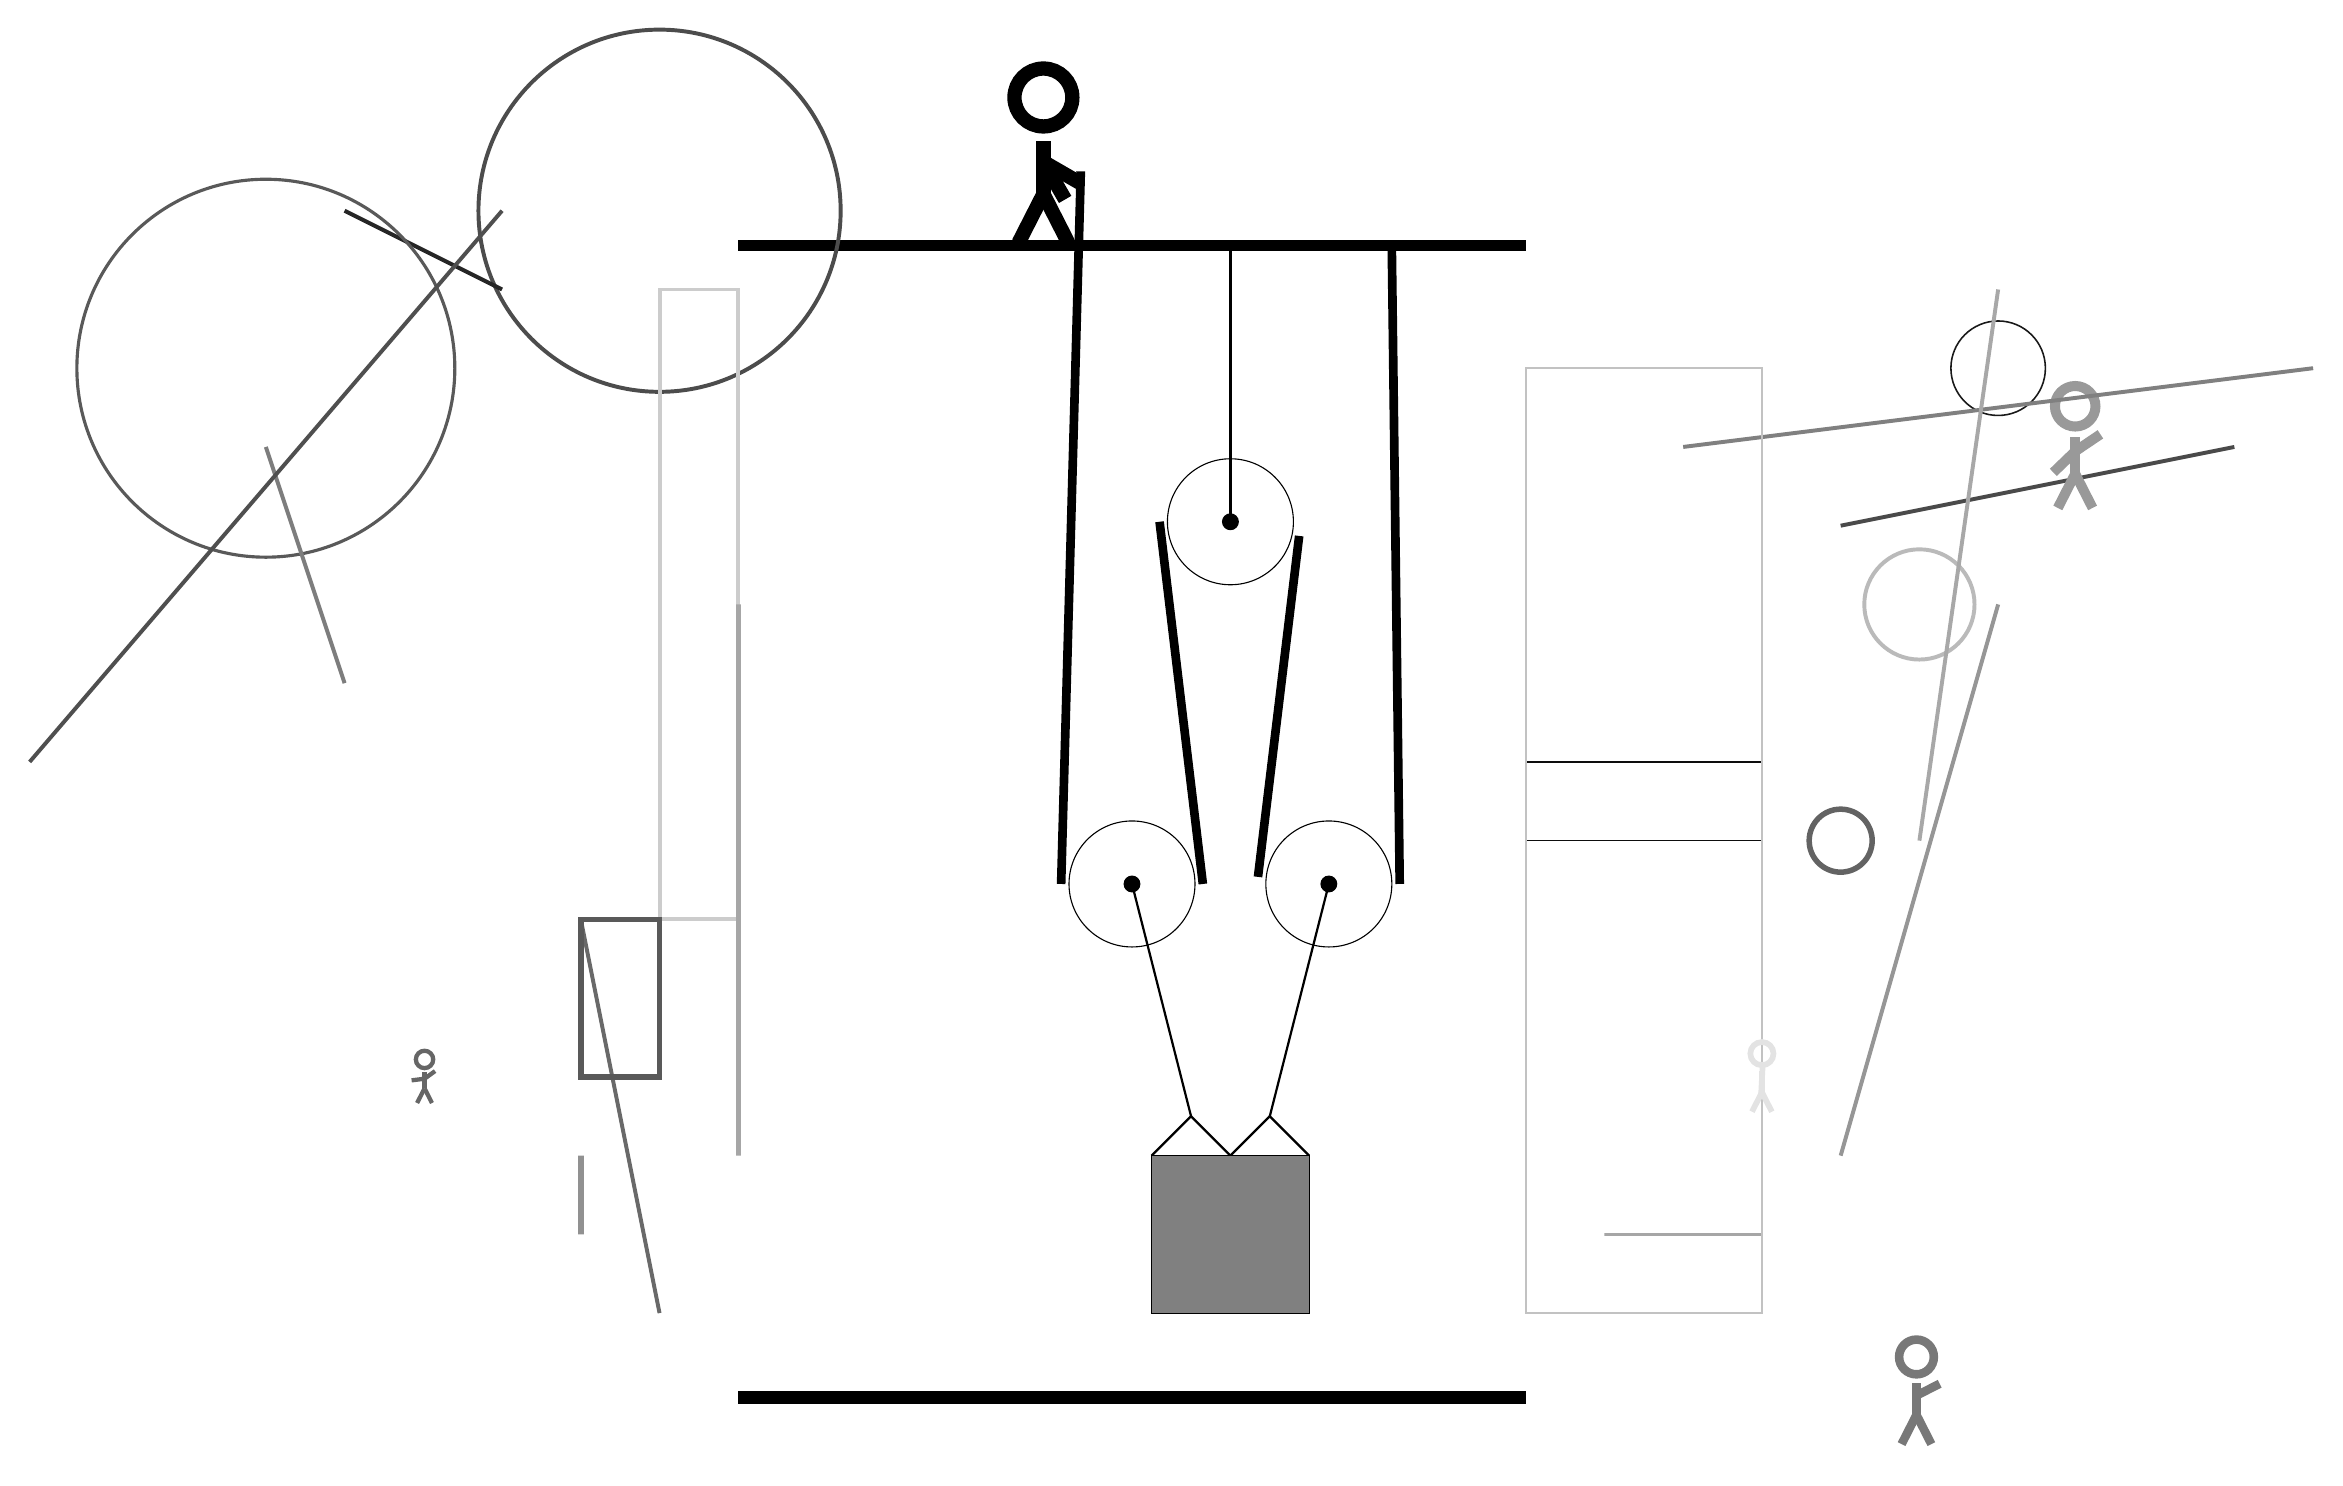
\begin{tikzpicture}
			%%%%% START %%%%%
			
			\draw[fill=black] (-4, 11.5) rectangle (6, 11.625);
			
			\draw (1, 3.45) circle (0.8);
			\draw[fill=black] (1, 3.45) circle (0.1);
			
			\draw (2.25, 8.05) circle (0.8);
			\draw[fill=black] (2.25, 8.05) circle (0.1);
			\draw[thick] (2.25, 8.05) -- (2.25, 11.5);
			
			\draw [line width=0.5mm, color=black!70](-5, 12) circle (2.3);
			
			\draw [line width=0.5mm, color=black!27](11, 7) circle (0.7);
			\draw[line width=0.4mm, color=black!35] (7, -1) rectangle (9, -1);
			\node[line width=0.2mm, color=black!53] at (11, -3) {\Strichmaxerl[6][90][27]};
			
			\draw[line width=0.2mm, color=black!95] (6, 5) rectangle (9, 4);
			\draw [line width=0.2mm, color=black!90](12, 10) circle (0.6);
			\draw[line width=0.7mm, color=black!43] (-6, 0) rectangle (-6, -1);
			\draw[line width=0.5mm, color=black!20] (-4, 3) rectangle (-5, 11);
			\draw [line width=0.7mm, color=black!61](10, 4) circle (0.4);
			\draw[line width=0.5mm, color=black!71](10, 8) -- (15, 9);
			
			\draw[line width=0.5mm, color=black!59](-5, -2) -- (-6, 3);
			
			\node[line width=0.6mm, color=black!40] at (13, 9) {\Strichmaxerl[7][44][34]};
			\draw[line width=0.5mm, color=black!85](-7, 11) -- (-9, 12);
			\draw[line width=0.5mm, color=black!41](10, 0) -- (12, 7);
			\draw [line width=0.4mm, color=black!65](-10, 10) circle (2.4);
			\draw[line width=0.5mm, color=black!50](8, 9) -- (16, 10);
			
			\draw[line width=0.7mm, color=black!65] (-6, 3) rectangle (-5, 1);
			\draw[line width=0.5mm, color=black!51](-9, 6) -- (-10, 9);
			\draw[line width=0.7mm, color=black!35] (-4, 0) rectangle (-4, 7);
			\node[line width=0.5mm, color=black!60] at (-8, 1) {\Strichmaxerl[3][7][36]};
			\draw[line width=0.3mm, color=black!24] (6, 10) rectangle (9, -2);
			\draw[line width=0.5mm, color=black!34](11, 4) -- (12, 11);
			
			\draw[line width=0.5mm, color=black!69](-7, 12) -- (-13, 5);
			\node[line width=0.7mm, color=black!11] at (9, 1) {\Strichmaxerl[4][87][87]};
			
			\draw (3.5, 3.45) circle (0.8);
			\draw[fill=black] (3.5, 3.45) circle (0.1);
			
			\draw[thick] (3.5, 3.45) -- (2.75, 0.5);
			\draw[thick] (1, 3.45) -- (1.75, 0.5);
			\draw[thick]  (1.25, 0) -- (1.75, 0.5) -- (2.25, 0);
			\draw[thick]  (2.25, 0) -- (2.75, 0.5) -- (3.25, 0);
			\draw[fill=black!50] (1.25, 0) rectangle (3.25, -2);
			
			\draw[line width=1.1mm] (0.35, 12.5) --  (0.1, 3.45);
			\centerarc[line width=1.1mm](1, 3.45)(180:360:0.9);
			\draw[line width=1.1mm] (1.9, 3.45) -- (1.35, 8.05);
			\centerarc[line width=1.1mm](2.25, 8.05)(-20:180:0.9);
			\draw[line width=1.1mm](3.123, 7.87) -- (2.6, 3.54);
			\centerarc[line width=1.1mm](3.5, 3.45)(160:360:0.9);
			\draw[line width=1.1mm](4.4, 3.45) -- (4.3, 11.5);
			
			\node at (-0.07, 12.7) {\Strichmaxerl[10][120][-30]};
			
			\draw[fill=black] (-4, -3) rectangle (6, -3.15);
			
			%%%%% END %%%%%
		\end{tikzpicture}
	\end{figure}	
\end{document}